\documentclass{beamer}
\usecolortheme{dolphin}
\usepackage{graphics}
\usepackage{graphicx}
\usepackage{listings}
\usepackage{amsmath}
\usepackage{fancyvrb}
\usepackage{color}
\usepackage[ascii]{inputenc}

\lstset{language=Python,
        keywordstyle=\color[rgb]{0,0,1},
        commentstyle=\color[rgb]{0.133,0.545,0.133},
        stringstyle=\color[rgb]{0.627,0.126,0.941},
        columns=fixed,}

\title{Parallelizing the Viterbi Algorithm in Python using PyCUDA and PP}
\subtitle{Project Presentation}
\author{Jon Klein}
\institute{University of Alaska, Fairbanks}
\date{December 14, 2011}

\begin{document}
    \begin{frame}
        \titlepage
    \end{frame}

    \begin{frame}
        \frametitle{Pyterbi is a parallelized Viterbi decoder written in Python}
        \begin{itemize}
            \item Pyterbi is parallelized for SMP and cluster computing using PP.
            \item Pyterbi is parallelized for Nvidia graphics cards using PyCUDA. 
            \item Pyterbi provides a roughly 100 times speedup over the reference implementation.
        \end{itemize}
    \end{frame}
 
    \begin{frame}
        \frametitle{The Viterbi Algorithm}
        The Viterbi algorithm finds the most likely sequence of states given the outputs.
        It is used for pattern recognition, error-correcting codes, and detecting signals with memory [1].

        \begin{figure}
            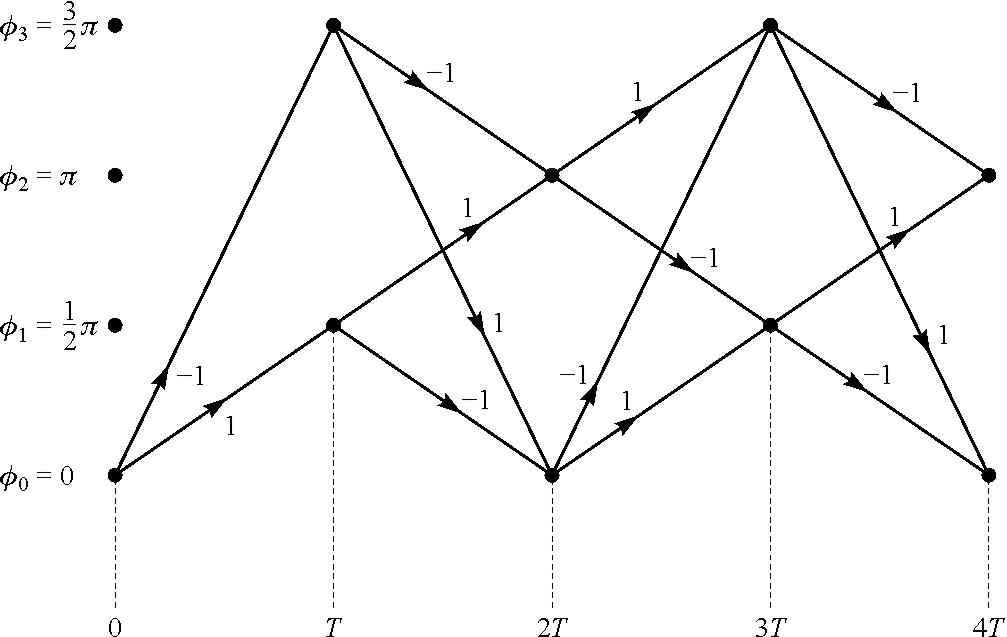
\includegraphics[options]{figures/cpmfulltrellis.jpg}
            \caption{Trellis diagram of $\frac{\pi}{2}$ full response CPM [2]}
        \end{figure}

    \end{frame}
    
    \begin{frame}
        \frametitle{The Viterbi algorithm is parallelizable}
        
        \begin{itemize}
            \item The path leading to a state depends on calculating the path to all previous states. However, the probability of each state at a moment in time can be calculated in parallel.
            \item The Viterbi algorithm can be run on multiple sequences in parallel.
            \item Many of the inputs are constant between between iterations, and can be left on device memory.
            \item Pyterbi makes each state a thread, and each trellis a grid.
        \end{itemize} 
    \end{frame}
    
    \begin{frame}
        \frametitle{The probability of each state depends only on the previous states}
        \begin{figure}
            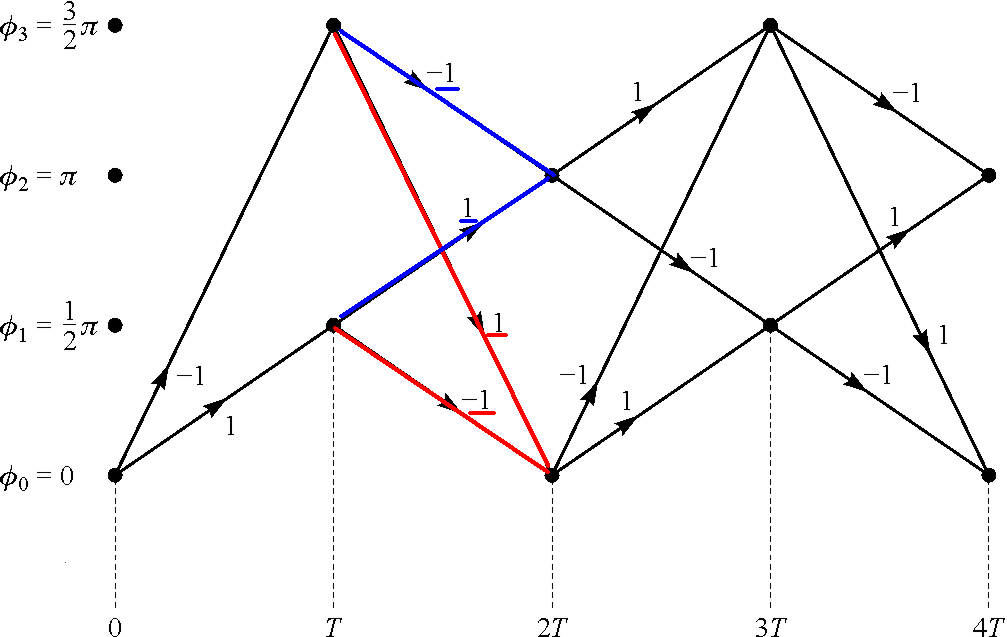
\includegraphics[width=.8\textwidth]{figures/cpmfulltrelliscolored.png}
            \caption{Decoding trellis diagram at time T=2Ts}
        \end{figure}
    \end{frame}
   
    \begin{frame}
    \frametitle{I tried several ways of optimizing the CUDA algorithm..}
    \begin{itemize}
        \item Moving constant matricies from global to constant memory pause slows down execution time by 50\%
        \item Moving less than 8kB of data to constant memory speeds up execution time by 5\%
        \item Caching matricies in shared memory speeds up execution time by another 5\%
        \item Reducing communication between the host and devices provides a ~120\% speedup.
        \item Discarding intermediate values of to reduce shared memory consumption.
        \item Coalescing global memory accesses.
        \item Parallelizing the backtrace.
    \end{itemize}
    These improvements increased the speedup from 15 to 100.
    \end{frame}

    \begin{frame}
        \frametitle{CUDA parallelized pyterbi is at least an order of magnitude faster than the host}
        \begin{figure}
            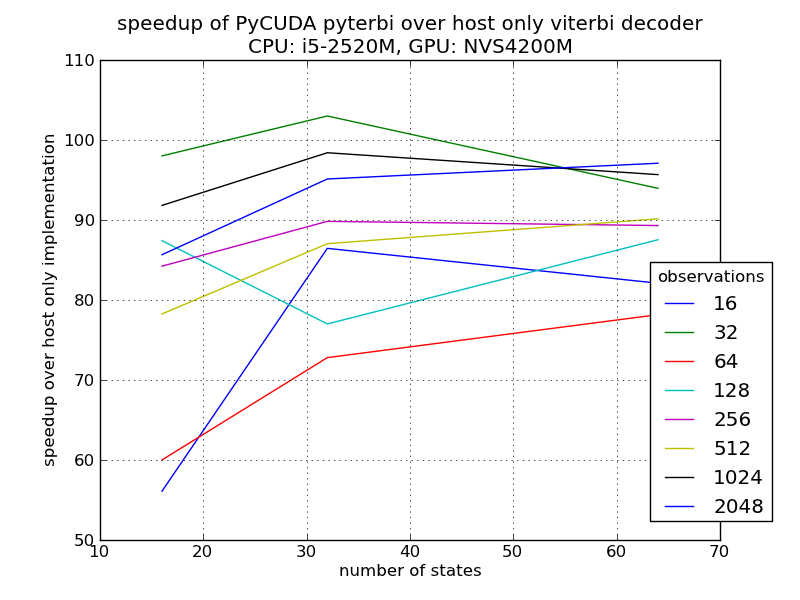
\includegraphics[width=.8\textwidth]{figures/speedupgraphcuda.png}
            \caption{Speedup from parallelizing viterbi algorithm using CUDA}
        \end{figure}

    \end{frame}
 
% bah, I can't indent this
\begin{frame}[fragile]
\frametitle{PP is an easy to use parallel programming python module}
PP is a Python module for cross-platform execution of Python on SMP and clusters. It has dynamic load balancing, fault-tolerance, and autodiscovery. 

\begin{figure}
\tiny
\begin{lstlisting}
import pp, hashlib 

def check(h, start, step):
    for n in xrange(start, start+step):
        if(hashlib.sha224(str(n)).digest() == h):
            return n

h = hashlib.sha224("1729").digest()
stop, step = 8000, 200

% create a job server
job_server = pp.Server(ppservers=("*",))
jobs = []

% create jobs to check a range of numbers in step chunks
for i in range(1, stop, step):
    jobs.append(job_server.submit(check, (h, i, step), (), ("hashlib",)))

% check results of jobs
for result in [j() for j in jobs]:
    if(result): print result

\end{lstlisting}
\caption{A parallelized SHA224 brute forcer in PP} 
\end{figure}
\end{frame}

   
    \begin{frame}
        \frametitle{SMP parallelized pyterbi will speedup sufficently complex workloads}
        Pyterbi uses the PP Python library to parallize pyterbi by creating a job for each trellises. 
        \begin{figure}
            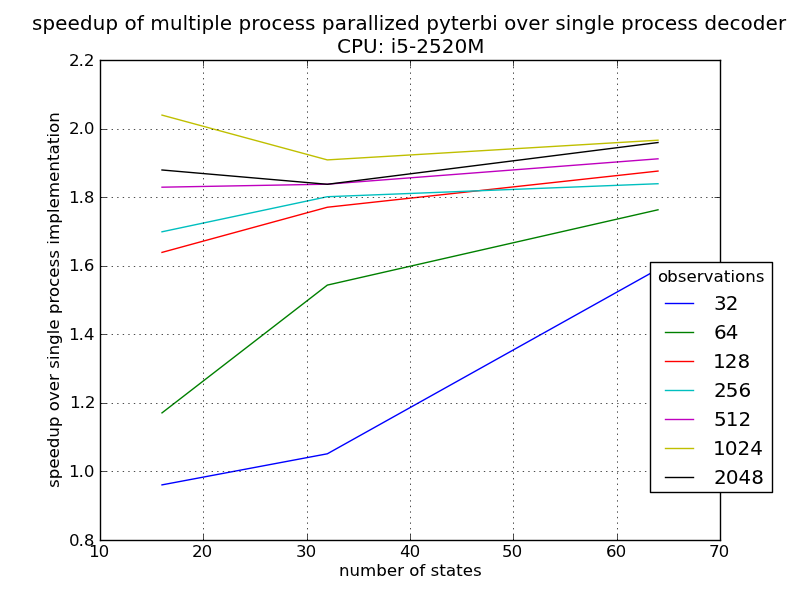
\includegraphics[width=.8\textwidth]{figures/speedupgraphhost.png}
            \caption{Speedup from parallelizing viterbi algorithm using SMP}
        \end{figure}

    \end{frame}
    
    \begin{frame}
        \frametitle{I ran the benchmarks on a non-ideal platform..}
        \begin{itemize}
            \item The processor speed scaled back to avoid overheating.
            \item The graphics card was also driving displays.
            \item Intel TurboBoost permits higher clock frequencies for single core applications.
        \end{itemize}

         \begin{columns}[t]
            \begin{column}[t]{.5\linewidth}
            \begin{block}{Host Specifications}
            \begin{itemize}
                \item Intel i5-2520M, 2.50GHz
                \item 3MB Cache
                \item 2 Hyper-Threaded cores
                \item 4096MB RAM
                \item Ubuntu 11.04
            \end{itemize}
            \end{block}
            \end{column}
            
            \begin{column}[t]{.5\linewidth}
            \begin{block}{Graphics Card}
            \begin{itemize}
                \item Nvidia NVS 4200M  
                \item 48 CUDA Cores
                \item Compute Capability 2.1
                \item 1.6 GHz GPU Clock
                \item 64-bit  Memory Bus
                \item 3000MB/s Host to Device Bandwidth 
                \item 2600MB/s Device to Host Bandwidth
            \end{itemize}
            \end{block}
            \end{column}
        \end{columns}
     

    \end{frame}

    \begin{frame}
        \frametitle{Cluster parallelized Viterbi works, but doesn't make sense..}
        Pyterbi gets a 10\% speedup by including a distant slow node.      
        \begin{columns}[t]
            \begin{column}[t]{.5\linewidth}
            \begin{block}{Node 1}
            \begin{itemize}
                \item Intel i5-2520M, 2.50GHz
                \item 4096MB RAM
                \item Tethered on AT\&T Cell Phone
                \item Ubuntu 11.04
                \item Fairbanks, Alaska
            \end{itemize}
            \end{block}
            \end{column}
            
            \begin{column}[t]{.5\linewidth}
            \begin{block}{Node 2}
            \begin{itemize}
                \item Shared 2.00 GHz AMD Opteron
                \item 192MB RAM
                \item 5 MBps Uplink
                \item Ubuntu 11.04
                \item VPS in New Jersey
            \end{itemize}
            \end{block}
            \end{column}
        \end{columns}
    \end{frame}

    \begin{frame}
        \frametitle{Project Results}
        I have written, tested, and benchmarked:
        \begin{itemize}
            \item a reference host-only implementation of the Viterbi algorithm in Python. 
            \item a CUDA parallelized Viterbi algorithm.
            \item a multi-process and cluster parallelized Viterbi implementation 
        \end{itemize}

        The pyterbi and presentation source code is available at: \texttt{http://github.com/loxodes/pyterbi}
   \end{frame}

   \begin{frame}
        There are some possible improvements remaining for pyterbi:
        \begin{itemize}
            \item Rewrite host code in a faster language (C)
            \item Rewrite host code for finer-grained parallelism
            \item Test kernel concurrency on more powerful graphics cards 
            \item Test realistic cases of cluster computing
            \item Get pycuda working with PP for CUDA accelerated cluster computations
        \end{itemize}
    \end{frame}

    \begin{frame}
        \frametitle{References}
        \begin{enumerate}
            \item Lou, H.-L.; , ``Implementing the Viterbi algorithm,'' Signal Processing Magazine, IEEE , vol.12, no.5, pp.42-52, Sep 1995
            \item John Proakis. Digital Communications. McGraw-Hill Science/Engineering/Math, 5 edition, 2007.
            \item C. Liu, ``CuHMM: a CUDA Implementation of Hidden Markov Model Training and Classification,'' 2009 
            \item Vanovschi V., ``Parallel Python Software,'', 2011, \texttt{http://www.parallelpython.com}
            \item Andreas Kloeckner, ``PyCUDA,'', 2011, \texttt{http://mathema.tician.de/software/pycuda}

        \end{enumerate}
    \end{frame}
\end{document}
